% !TeX spellcheck = en_US
%% 字体:方正静蕾简体
%%		 方正粗宋
\documentclass[a4paper,left=2.5cm,right=2.5cm]{article}

\usepackage[utf8]{inputenc}
\usepackage{fontspec}
\usepackage{cite}
\usepackage{xeCJK}
\usepackage{indentfirst}
\usepackage{titlesec}
\usepackage{longtable}
\usepackage{graphicx}
\usepackage{float}
\usepackage{rotating}
\usepackage{subfigure}
\usepackage{tabu}
\usepackage{amsmath}
\usepackage{setspace}
\usepackage{amsfonts}
\usepackage{appendix}
\usepackage{listings}
\usepackage{xcolor}
\usepackage{geometry}
\setcounter{secnumdepth}{4}
\titleformat*{\section}{\LARGE}
\renewcommand\refname{参考文献}
%\titleformat{\chapter}{\centering\bfseries\huge\wryh}{}{0.7em}{}{}
%\titleformat{\section}{\LARGE\bf}{\thesection}{1em}{}{}
\titleformat{\subsection}{\Large\bfseries}{\thesubsection}{1em}{}{}
\titleformat{\subsubsection}{\large\bfseries}{\thesubsubsection}{1em}{}{}
\renewcommand{\contentsname}{{\cjkfzcs \centerline{目{  } 录}}}
\setCJKfamilyfont{cjkhwxk}{华文行楷}
%\setCJKfamilyfont{cjkfzcs}{方正粗宋简体}
\newcommand*{\cjkfzcs}{\CJKfamily{cjkfzcs}}
\newcommand*{\cjkhwxk}{\CJKfamily{cjkhwxk}}
\newfontfamily\wryh{Microsoft YaHei}
%\newfontfamily\ygyfryg{叶根友福荣银钩}
\newfontfamily\hwzs{华文中宋}
\newfontfamily\hwst{华文宋体}
\newfontfamily\hwfs{华文仿宋}
%\newfontfamily\jljt{方正静蕾简体}
\newfontfamily\hwxk{华文行楷}
\newcommand{\verylarge}{\fontsize{60pt}{\baselineskip}\selectfont}  
\newcommand{\chuhao}{\fontsize{44.9pt}{\baselineskip}\selectfont}  
\newcommand{\xiaochu}{\fontsize{38.5pt}{\baselineskip}\selectfont}  
\newcommand{\yihao}{\fontsize{27.8pt}{\baselineskip}\selectfont}  
\newcommand{\xiaoyi}{\fontsize{25.7pt}{\baselineskip}\selectfont}  
\newcommand{\erhao}{\fontsize{23.5pt}{\baselineskip}\selectfont}  
\newcommand{\xiaoerhao}{\fontsize{19.3pt}{\baselineskip}\selectfont} 
\newcommand{\sihao}{\fontsize{14pt}{\baselineskip}\selectfont}      % 字号设置  
\newcommand{\xiaosihao}{\fontsize{12pt}{\baselineskip}\selectfont}  % 字号设置  
\newcommand{\wuhao}{\fontsize{10.5pt}{\baselineskip}\selectfont}    % 字号设置  
\newcommand{\xiaowuhao}{\fontsize{9pt}{\baselineskip}\selectfont}   % 字号设置  
\newcommand{\liuhao}{\fontsize{7.875pt}{\baselineskip}\selectfont}  % 字号设置  
\newcommand{\qihao}{\fontsize{5.25pt}{\baselineskip}\selectfont}    % 字号设置 

\usepackage{diagbox}
\usepackage{multirow}
\boldmath
\XeTeXlinebreaklocale "zh"
\XeTeXlinebreakskip = 0pt plus 1pt minus 0.1pt
\definecolor{cred}{rgb}{0.8,0.8,0.8}
\definecolor{cgreen}{rgb}{0,0.3,0}
\definecolor{cpurple}{rgb}{0.5,0,0.35}
\definecolor{cdocblue}{rgb}{0,0,0.3}
\definecolor{cdark}{rgb}{0.95,1.0,1.0}
\lstset{
	language=matlab,
	numbers=left,
	numberstyle=\tiny\color{black},
	showspaces=false,
	showstringspaces=false,
	basicstyle={\footnotesize}\ttfamily,
	keywordstyle=\color{cdocblue}\bfseries,
	commentstyle=\color{cgreen},
	stringstyle=\color{cred},
	frame=lines,
	escapeinside=``,
	xleftmargin=1em,
	xrightmargin=1em, 
	%backgroundcolor=\color{cdark},
	aboveskip=1em,
	breaklines=true,
	tabsize=4
} 

\newfontfamily{\consolas}{Consolas}
\newfontfamily{\monaco}{Monaco}
\setmonofont[Mapping={}]{Consolas}	%英文引号之类的正常显示,相当于设置英文字体
\setsansfont{Consolas} %设置英文字体 Monaco, Consolas,  Fantasque Sans Mono
\setmainfont{Times New Roman}

\setCJKmainfont{华文中宋}

\newcommand*{\mytitle}
{
	
	\begingroup 
	\begin{center}
		\vspace*{0.05\paperheight} % White space at the top of the page
		\rule{\textwidth}{1.6pt}\vspace*{-\baselineskip}\vspace*{2pt} % Thick horizontal line
		\rule{\textwidth}{0.4pt}\\[\baselineskip] % Thin horizontal line
		{\yihao{\cjkhwxk {数学软件——短学期课程 \\[0.4\baselineskip]Matlab第一次作业}}}\\[0.2\baselineskip] % Title
		\rule{\textwidth}{0.4pt}\vspace*{-\baselineskip}\vspace{3.2pt}		
		\rule{\textwidth}{1.6pt}\\[3\baselineskip]
		
\includegraphics[width=0.5\textwidth]{xiaohui.jpg}
		\vspace*{3\baselineskip} % Whitespace between 
		{\LARGE\hwzs
			\begin{longtable}{ll}
				\cjkfzcs{姓名:}& ***\\
				\cjkfzcs{学号:}& ***\\
				\cjkfzcs{班级:}& ***\\
			\end{longtable}
		}\par
		\vspace*{1\baselineskip}
		{\Large\hwzs 2016.07.08}
	\end{center}
	\vfill
	\endgroup
}
\usepackage{lastpage}
\usepackage{fancyhdr}
\pagestyle{fancy}
\lhead{\space \qquad \space}
\chead{数学软件——短学期课程 \qquad}
\rhead{\qquad\thepage/\pageref{LastPage}}
\begin{document}
	\begin{titlepage}
		\mytitle
	\end{titlepage}
	\begin{spacing}{1.1}
		
	\tableofcontents
	\end{spacing}
	\newpage
	\begin{spacing}{1.6}
		\section{按行三数组与全存储相互转换}
		\subsection{全存储转换为三数组}
		
		\subsubsection{算法分析}
		通过两个for循环将全矩阵转换为按行三数组存储模式,时间复杂度为$O(n^2)$,运行结果见图(\ref{full2sp}),转换结果的正确性可以通过后续运算过程体现出来
		\begin{figure}[H]
			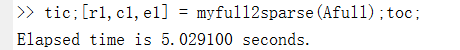
\includegraphics[width=0.9\textwidth]{image/full2sp.png}
			\caption{全存储转换为三数组}
			\label{full2sp}
		\end{figure}
		\subsubsection{代码}
		\lstinputlisting{code/myfull2sparse.m}
		\subsection{三数组转换为全存储}
		\subsubsection{算法分析}
		通过两个for循环,其中一个for循环对行遍历,然后第二个for循环对该行非零元素(含对角元)进行遍历。假设每行非零元分布大体均匀,于是时间复杂度为$O(n\times \frac{N}{n}) = O(N)$,考虑极端情况,时间复杂度为$O(n\times N)$。
		
		运行结果如图(\ref{sp2full})所示,转换结果的正确性可以通过后续运算过程体现出来。
			\begin{figure}[H]
				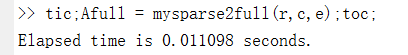
\includegraphics[width=0.9\textwidth]{image/mysp2full.png}
				\caption{三数组存储转换为全存储}
				\label{sp2full}
			\end{figure}
			\subsubsection{代码}
		\lstinputlisting{code/mysparse2full.m}
		\section{按行三数组与Matlab稀疏存储}
		\subsection{Matlab稀疏存储转换为按行三数组存储}
		\subsubsection{算法分析}
		首先通过对非零行元素从小到大排序,然后对非零元按行进行遍历进而online转换为三数组存储,对某行全空对对角元进行操作,因为是online的,所以可以判断时间复杂度为$O(n)$
		
		运行结果如图(\ref{matsp2sp})所示,转换结果的正确性可以通过后续运算过程体现出来。
		\begin{figure}[H]
			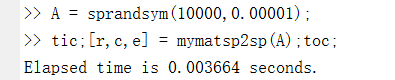
\includegraphics[width=0.9\textwidth]{image/matsp2sp.png}
			\caption{Matlab稀疏存储转换为行三数组存储}
			\label{matsp2sp}
		\end{figure}
		\subsubsection{代码}
		\lstinputlisting{code/mymatsp2sp.m}
		\subsection{按行三数组存储转换为Matlab稀疏存储}
		\subsubsection{算法分析}
		通过两个for循环,其中一个for循环对行遍历,另一个对每行的非零元(含对角元)历。设每行非零元分布大体均匀,于是时间复杂度为$O(n\times \frac{N}{n}) = O(N)$,考虑极端情况,时间复杂度为$O(n\times N)$。
		
		运行结果如图(\ref{sp2matsp})所示,转换结果的正确性可以通过后续运算过程体现出来。
		\begin{figure}[H]
			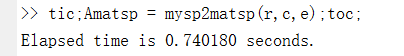
\includegraphics[width=0.9\textwidth]{image/sp2matsp.png}
			\caption{行三数组转换为Matlab稀疏存储}
			\label{sp2matsp}
		\end{figure}
		\subsubsection{代码}
		\lstinputlisting{code/mysp2matsp.m}
		\section{在指定位置添加非零元素}
		\subsection{算法分析}
		避免了使用for循环,采用矩阵运算(代码24,25行),故时间复杂度可以看作是$O(1)$。值得说明的是,这个函数还可以向已有非零元进行加法计算,这是为了方便后续矩阵加矩阵做铺垫。
		
		运行结果如图(\ref{add})所示,通过判断$C$与$A$是否相等来检验正确性
		\begin{figure}[H]
			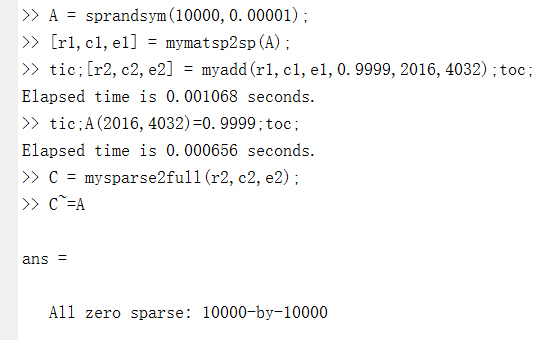
\includegraphics[width=0.9\textwidth]{image/add.png}
			\caption{添加非零元}
			\label{add}
		\end{figure}
		\subsection{代码}
		\lstinputlisting{code/myadd.m}
		\section{剔零压缩存储}
		\subsection{算法分析}
		避免了for循环,采用矩阵向量运算,于是可以将时间复杂度看成是$O(1)$。
		运行结果如下图(\ref{zero})所示,通过时间来看,这与上述时间复杂度的判断是一致的,而且结果是正确的。
		\begin{figure}[H]
			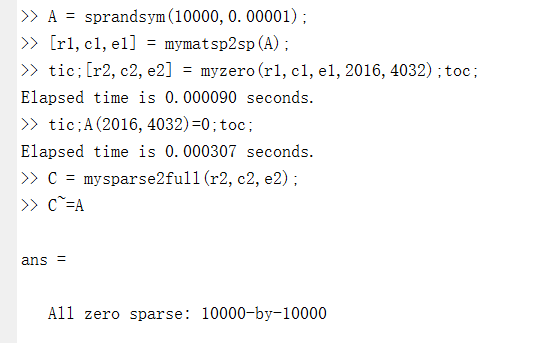
\includegraphics[width=0.9\textwidth]{image/zero.png}
			\caption{剔零压缩存储}
			\label{zero}
		\end{figure}
		\subsection{代码}
		\lstinputlisting{code/myzero.m}
		\section{矩阵加法}
		\subsection{算法分析}
		对第二个矩阵的非零元进行遍历,利用myadd.m先把第二个矩阵的每一个非零元插入第一个矩阵中,这里有两种情况,一是添加的元素在矩阵一中不为零(或是对角元),这种就相当于简单的在矩阵一中添加非零元;第二种情况是矩阵二中的元素在矩阵一中对应的元素非零(或为对角元),亦即在entries1中有相应的元素,这是利用在myadd.m中后一段代码便可以实现加法,同时还可以实现压缩存储。
		
		又因为myadd.m的时间复杂度为$O(1)$,myzero.m的时间复杂度为$O(1)$,则此时时间复杂度为$O(N_2)$,其中,$N_2$为第二个矩阵的非零元个数。
		
		运行结果如下图(\ref{plus})所示,通过判断$C1$与$C$是否相等,来判断运算结果的正确性。
		\begin{figure}[H]
			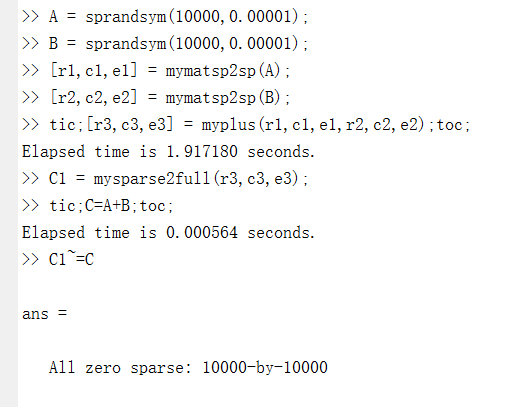
\includegraphics[width=0.9\textwidth]{image/plus.png}
			\caption{矩阵加法}
			\label{plus}
		\end{figure}
		\subsection{代码}
		\lstinputlisting{code/myplus.m}
		\section{矩阵减法}
		\subsection{算法分析}
		矩阵减法直接利用上述矩阵加法,故其时间复杂度也为$O(N_2)$。
		运行结果如下图(\ref{plus})所示
		\begin{figure}[H]
			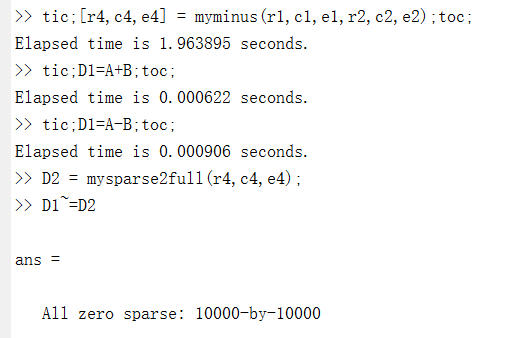
\includegraphics[width=0.9\textwidth]{image/minus_result.png}
			\caption{矩阵减法}
			\label{plus}
		\end{figure}
		\subsection{代码}
		\lstinputlisting{code/myminus.m}
		\section{矩阵乘向量}
		\subsection{算法分析}
		通过两个for循环,其中一个for循环对行遍历,另一个对每行的非零元(含对角元)遍历。设每行非零元分布大体均匀,于是时间复杂度为$O(n\times \frac{N}{n}) = O(N)$,考虑极端情况,时间复杂度为$O(n\times N)$
		
		对于$A\times b$,$A$为$10^4$阶方阵,$b$为$1\times 10^4$的行向量,结果如下图所示,可见虽然运算速度远不及matlab,但仍属于可接受的范围,而且运算结果是正确的。
		\begin{figure}[H]
			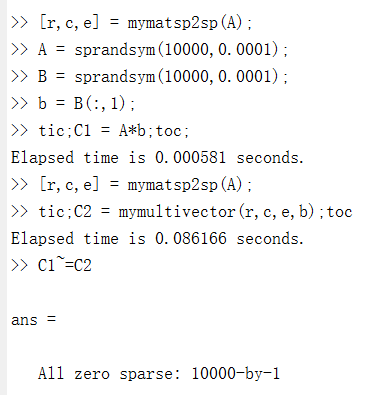
\includegraphics[width=0.9\textwidth]{image/multivector_result1.png}
		\end{figure}
		\subsection{代码}
		\lstinputlisting{code/mymultivector.m}
		%\section{向量乘矩阵}
		%这是为了后续矩阵乘矩阵做的铺垫,因为矩阵乘矩阵如果转换为矩阵乘向量不是很方便,因为是按行三数组存储稀疏矩阵,所以取矩阵的列不是很方便,所以我选择了一个过渡,先计算向量乘矩阵,然后再实现矩阵乘矩阵。
		
		%为了实现向量乘矩阵,我先计算转置,即矩阵乘向量,然后再转置回来。其中矩阵转置为$O(n^2)$
		
		%\lstinputlisting{code/myvectormulti.m}
		\section{矩阵乘矩阵}
		\subsection{算法分析}
		考虑矩阵$A\times B$,对矩阵$A$的行进行遍历,对矩阵的每一行中的非零元(含对角元),对于在矩阵$B$中的对应的行,找出非零元所在的列组成nonzerocol2,这样矩阵乘法只需要对矩阵$A$的每一行和nonzerocol2中的列进行运算,在非零元分布相对均匀时情况下,时间复杂度为$O(n\times \frac{N_1}{n} \times  \frac{N_2}{n}) = O(\frac{N_1N_2}{n})$,极端情况下,时间复杂度为$O(n\times N_1 \times N_2)$
		
		对于一万乘以一万,稀疏度为$10^{-4}$的矩阵,运行结果如下图(\ref{res1})所示。可见虽然效率跟matlab相比完全不在一个量级,但至少说得过去,毕竟matlab有一堆数学家在研究算法。
		\begin{figure}[H]
			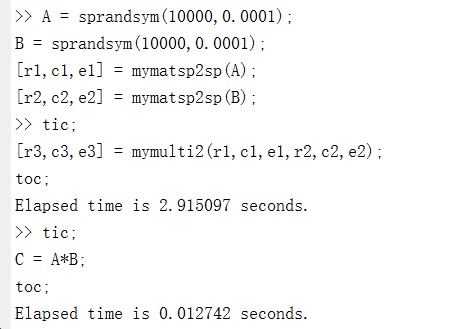
\includegraphics[width = 0.9\textwidth]{image/multi_result3.png}
			\caption{$10^4\times10^4$稀疏度为$10^{-4}$}
			\label{res1}
		\end{figure}
		下图(\ref{res2})展现了运算结果的正确性,因为没有元素是不相等的。
		\begin{figure}[H]
			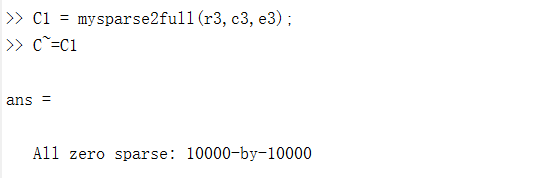
\includegraphics[width=0.9\textwidth]{image/multi_result2.png}
			\caption{检验结果是否正确}
			\label{res2}
		\end{figure}
		\begin{figure}[H]
			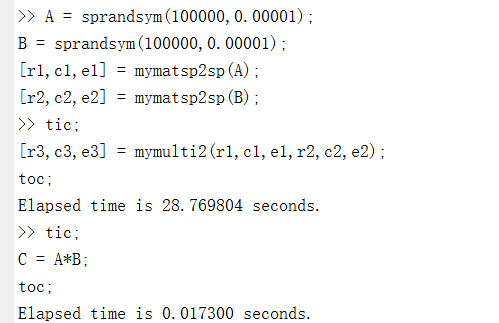
\includegraphics[width=0.9\textwidth]{image/multi_result1.png}
			\caption{挑战十万级别}
		\end{figure}
		挑战十万乘十万阶的矩阵
		发现还是可以运行的,虽然跟matlab的运行速度相差更大。
		\subsection{代码}
		\lstinputlisting{code/mymulti2.m}
	\end{spacing}
\end{document}
